%!TEX TS-program = xelatex
\documentclass[]{shiltemann-cv}
%\addbibresource{publications.bib}
\usepackage{fontspec}
\usepackage{verbatim}
\defaultfontfeatures{Path = /usr/share/texlive/texmf-dist/fonts/opentype/public/fontawesome/}
\usepackage{fontawesome}


\begin{document}
\header{Saskia}{Hiltemann}
    {Post-Doctoral Researcher, Bioinformatics \& Education}


% In the aside, each new line forces a line break
\begin{aside}
  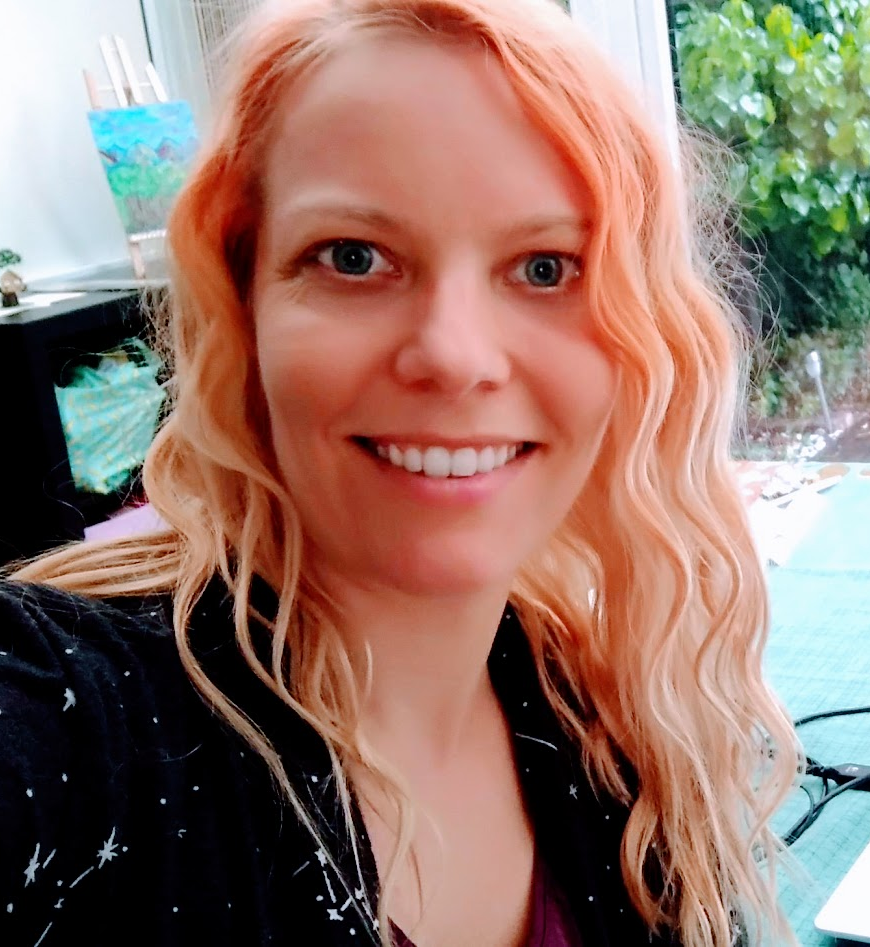
\includegraphics[width=75pt]{photo-saskia.png}
  \section{About}
    Saskia Hiltemann, Ph.D.
    ~
    Thérèse Schwartzestraat 24
    2597 XJ, Den Haag
    The Netherlands
    ~
    +31 6 33 951 365 \faPhone
    ~
    saskiahilltemann @gmail.com \faEnvelope
    @shiltemann \faGithub \ \faTwitter \ \faLinkedin
    \ \\
    ORCiD:
    0000-0003-3803-468X \faOrcid
  \section{Languages}
    Fluent: Dutch,English
    Some: German \& French
  \section{Tech Skills}
    Galaxy, UNIX, git, Jekyll, Python, C, C++, Docker, LaTeX, HTML, CSS, Javascript
  \section{Other Skills}
    Training, Community Building, Outreach \& Dissemination, Data Stewardship
\end{aside}

\section{Interests}

Bioinformatics, Education \& Training, Open Science, FAIR principles, Community Building, Data Stewardship, Genome Sequencing, Plant research, Cancer Research, Microbiome Analysis, Workflows, Automation, Visualisation, Best Practices, Infosec, CTF, Traveling, Hiking, Reading, Puzzles.


\section{Projects}
\emph{Selection of current and recent projects.}

\begin{entrylist}
   \entry
    {2023-current}
    {MAdLand Project}
    {Molecular Adaptation to Land: plant evolution to change}
    {MAdLand is a DFG priority programme investigating the molecular adaptations of plants from water to land. In the context of this project I am responsible for scientific tool development and data stewardship. I work closely together with the DataPLANT/NFDI4Plants consortium as well as the Freiburg Galaxy team. We are strongly committed to making all data and analysis workflows generated within the consortium available to the scientific community through the use of FAIR data initiatives such as DataPLANT ARCs.}

\end{entrylist}

\begin{entrylist}
    \entry
    {2015-current}
    {Galaxy Training Network (GTN): Training Materials, Infrastructure \& Community Building}
    {GalaxyProject}
    {Co-founder of the GTN platform for the collaborative development of data science training materials. Software development \& community building efforts to ensure sustainability of the project, utility for educators, and integrations with FAIR data initiatives. Development of numerous data science tutorials. https://training.galaxyproject.org }
\end{entrylist}


\begin{entrylist}
   \entry
    {2020-2023}
    {Gallantries Project: Project Coordinator \& Work Package Lead}
    {ErasmusMC, Erasmus+ KA203 grant}
    {Development of bioinformatics curricula for higher education and workshops for later-career researchers. Building of training infrastructure for educators, with a focus on remote training.}
\end{entrylist}

\begin{entrylist}
   \entry
    {2019-2023}
    {CINECA project: Work Package co-lead, Training \& Dissemination}
    {ErasmusMC, Horizon2020 grant}
    {CINECA (Common Infrastructure for National Cohorts in Europe, Canada, and Africa) aims to create a global infrastructure for federated data analysis. Co-lead of the Training \& Dissemination  work package, technical lead of the Healthcare Interoperability \& Clinical Applications work package.}
 \end{entrylist}





\section{Publications}
\emph{Selection of scientific publications.}

\begin{entrylist}

\entry
  {2024}
  {FAIR data retrieval for sensitive clinical research data in Galaxy }
  {Giga Science}
  {DOI: 10.1093/gigascience/giad099}

\end{entrylist}
\begin{entrylist}

\entry
  {2023}
  {Galaxy Training: A powerful framework for teaching!}
  {PLOS Computational Biology}
  {DOI: 10.1371/journal.pcbi.1010752 }

\end{entrylist}

\begin{entrylist}

\entry
  {2022}
  {FAIR Genomes metadata schema promoting Next Generation Sequencing data reuse in Dutch healthcare and research}
  {Nature Scientific Data}
  {DOI: 10.1038/s41597-022-01265-x}
\end{entrylist}

%\begin{entrylist}

%\entry
%  {2020}
%  {Galactic Circos: User-friendly Circos plots within the Galaxy platform}
%  {GigaScience}
%  {DOI: 10.1093/gigascience/giaa065}

%\end{entrylist}
\begin{entrylist}

\entry
  {2019}
  {Galaxy mothur Toolset (GmT): a user-friendly application for 16S rRNA gene sequencing analysis using mothur}
  {GigaScience}
  {DOI: 10.1093/gigascience/giy166}

\end{entrylist}

\begin{entrylist}
\entry
 {2018}
 {Community-driven data analysis training for biology}
 {Cell Systems}
 {DOI: 10.1016/j.cels.2018.05.012}
\end{entrylist}

\begin{entrylist}
\entry
  {2018}
  {Development and evaluation of a culture-free microbiota profiling platform (MYcrobiota) for clinical diagnostics}
  {European Journal of Clinical Microbiology \& Infectious Diseases}
  {DOI: 10.1007/s10096-018-3220-z}
\end{entrylist}

%\begin{entrylist}
%\entry
%  {2017}
%  {ASaiM: a Galaxy-based framework to analyze raw shotgun data from microbiota}
%  {GigaScience}
%  {DOI: 10.1093/gigascience/giy057}
%\end{entrylist}

%\begin{entrylist}

%\entry
%  {2015}
%  {Discriminating somatic and germline mutations in tumor DNA samples without matching normals }
%  {Genome Research}
%  {DOI: 10.1101/gr.183053.114}

%\end{entrylist}

%\begin{entrylist}

%\entry
%  {2014}
%  {iReport: a generalised Galaxy solution for integrated experimental reporting}
%  {GigaScience}
%  {DOI: 10.1186/2047-217X-3-19}
%\end{entrylist}

For a full list of publications, please see ORCiD: \url{https://orcid.org/0000-0003-3803-468X}

\section{Community Activities}
\begin{entrylist}

\entry
  {ongoing}
  {ELIXIR Europe: A European life sciences infrastructure}
  {Galaxy Working Group}
  {Foster the use and development of Galaxy withing the ELXIR Europe community, focusing on making it easier to import data into Galaxy instances, helping to develop and share Galaxy tools and workflows, and increasing the provision of Galaxy training.}
\end{entrylist}

\begin{entrylist}
\entry
  {ongoing}
  {MicroGalaxy Community}
  {Community Building, tool development, workflow development, training, FAIR science }
  {Creating a community around microbial research in Galaxy. Identifying needs of the community and developing solutions to address those needs. Democratizing resources (e.g. tools, databases) for microbial research communities.}

\end{entrylist}
\begin{entrylist}

\entry
  {ongoing}
  {Galaxy Intergalactic Utilities Commission (IUC) member}
  {Galaxy Tool development}
  {Best-practice Galaxy tool development and maintenance. Creating best-practice guidelines to ensure \emph{FAIRness} of tools and workflows as well as integrations with existing FAIR science initiatives.}

\end{entrylist}

\begin{entrylist}
\entry
  {ongoing}
  {GalaxyProject Outreach, Training \& Support}
  {Galaxy Working Group}
  {Member of the GalaxyProject Outreach, Training \& Support working group. Coordinating Training and outreach activities for the GalaxyProject and its global community of stakeholders}
\end{entrylist}

\begin{entrylist}
\entry
  {ongoing}
  {F1000Research Galaxy Gateway}
  {Advisory Board Member}
  {Provide strategic input on F1000Research directions, with a focus on Galaxy-related publications}
  {}
\end{entrylist}


\begin{comment}
\section{Grants}
Selection of grants obtained.

\begin{entrylist}

\entry
  {2020}
  {Gallantries Project}
  {Erasmus+ Programme of the European Union}
  {Grant number KA203, 2020-1-NL01-KA203-064717 \url{https://gallantries.github.io/}}

\end{entrylist}
\begin{entrylist}

\entry
  {2019}
  {Cineca Project}
  {Horizon 2020}
  {Grant Agreement No 825775, \url{https://www.cineca-project.eu/} }

\end{entrylist}
\begin{entrylist}

\entry
  {2019}
  {Gallantries Pilot Project}
  {Mozilla Open Science Awards}
  {Mini-grant. \url{https://medium.com/read-write-participate/meet-mozillas-latest-open-science-awardees-cfa45348e5d5#7d0f}}
\end{entrylist}
\end{comment}

\section{Employment History}

\begin{entrylist}
 \entry
    {2024-current}
    {RPTU - Rheinland-Pfälzische Technische Universität Kaiserslautern}
    {Computational Systems Biology group, Department of Biology}
    {Post-doctoral Researcher \& Bioinformatician
    \begin{itemize}
      \item Data stewardship
      \item DataPLANT/NFDI4Plants member
      \item Scientific software development
    \end{itemize}}


 \entry
    {2023-current}
    {Albert-Ludwigs-Universität Freiburg}
    {Institute of Pharmaceutical Sciences, Faculty of Chemistry and Pharmacy}
    {Post-doctoral Researcher \& Bioinformatician
    \begin{itemize}
      \item Scientific software development
      \item Data stewardship
      \item Galaxy tool and workflow development
      \item Galaxy Training Network lead
    \end{itemize}}
 \entry
    {2012-2023}
    {Erasmus Medical Center, Rotterdam}
    {Clinical Bioinformatics group, Department of Pathology}
    {Post-doctoral Researcher \& Bioinformatician
     \begin{itemize}
       \item \emph{Galaxy tool and workflow development}
       \item \emph{Education \& Curriculum Development}
       \item \emph{Microbiota Analysis and Antibiotic Resistance Detection}
       \item \emph{Prostate Cancer Analysis}
       \item \emph{Software Development and Pipeline building}
       \item \emph{Galaxy System's Administrator}
       \item \emph{Training, Outreach \& Dissemination}
       \item \emph{Federated Data Analysis Infrastructure Development}
       \item \emph{FAIR data analysis}
     \end{itemize}}
  \entry
    {2010-2012}
    {After's Cool, The Hague}
    {Part-time science tutoring}
    {Tutor of High School Students. \emph{Math, Physics, Chemistry}}
\end{entrylist}


\section{Education}

\begin{entrylist}
  \entry
    {2021}
    {Ph.D. Bioinformatics}
    {Erasmus Medical Center}
    {\emph{Thesis:} "Jigsaw Genomics: Assembling the pieces toward open and accessible bioinformatics for everyone"}
\end{entrylist}
\begin{entrylist}


  \entry
    {2010}
    {M.Sc.}
    {LIACS, University of Leiden \& TU Delft}
    {Computer Science, Specialization in Bioinformatics}

\end{entrylist}
\begin{entrylist}

  \entry
    {2008}
    {B.Sc.}
    {LIACS, University of Leiden}
    {Computer Science}
\end{entrylist}
\begin{entrylist}


  \entry
    {2002–2005}
    {B.Sc. course work}
    {University of Leiden}
    {Physics \& Astronomy}
\end{entrylist}
\begin{entrylist}


  \entry
    {2002}
    {High School (VWO)}
    {Alfrink College, Zoetermeer}
    {Specialization in Science \& Technology}
\end{entrylist}



\end{document}
